\documentclass{article}
\usepackage[colorlinks=true, allcolors=blue]{hyperref}
\usepackage{graphicx}
\usepackage{amsmath}
\usepackage[margin=1in]{geometry}

% Full tokenomic visualization/simulation.

\title{Revnets}
\author{Filip\\f@filip.world}

\begin{document}
\maketitle

\section{Introduction}

Successful organizational frameworks have always been well-adapted to the technologies of their respective eras. In our current era of internet-native business and user-generated value, many frameworks have grown anachronistic, failing to optimally align participants:

\begin{enumerate}
  \item Companies operating under a shareholder value model are obligated to prioritize profit-making, efficiency, and market competitiveness, even at the expense of their customers' interests. Companies often use funds from investors to undercut competition and secure a dominant market position, at which point they move to increasingly extractive revenue models to secure profits, trapping users in a more expensive ecosystem. Shareholder value models can also lead to misalignments between shareholder and employee interests---shareholders (particularly institutional investors and activist shareholders) tend to prefer shorter growth horizons over longer ones, compensation tied to stock performance over predictable salaries, and often support mergers and acquisitions even when disruptive, whereas employees tend to prefer the opposite. This time horizon mismatch often leads to conflicts over investments in R\&D, training, and other long-term growth initiatives, contributing to the stagnation of larger companies which can fall behind smaller competitors.
  \item Decentralized autonomous organizations (DAOs) pose an alternative, but frequently fall short in practice. Most DAOs begin with a core group of founders, developers, and entrepreneurs who aim to expand the DAO through progressive decentralization. Operating a DAO and pursuing decentralization is often time-consuming and resource intensive, and does not further the development of the end product. These projects can create a false sense of product market fit, where users will adopt a product with the hope of eventually receiving a token airdrop. Once this airdrop finally takes place, these users generally sell their tokens and leave the community. Progressive decentralization also disadvantages users and investors who must contend with the risk of misalignment, rugpulls, and scams while a core team holds significant power.
  \item Stakeholder capitalism and triple bottom line models may be beneficial in theory, but frequently fail to align individual incentives and become difficult to enforce in practice.
\end{enumerate}

Revnets utilize an alternative framework\footnote{\href{https://jango.eth.limo/9E01E72C-6028-48B7-AD04-F25393307132}{Retailism}.} under which wealth is programmatically exchanged over time from newer participants to older ones. Revnets incentivize investors, customers, and builders in the same way---debt is predictably passed from one generation of voluntary participants to the next. A Revnet's product may not be free, but the Revnet model drives consumer costs towards zero, or even profitability as the network achieves scale, meaning the network does not need to orient towards excessive retail extraction. Revnets are implemented as ownerless Ethereum smart contracts, removing the need for governance and making most kinds of rugpulls and scams impossible.

Under the shareholder value model, surplus is returned to investors, meaning employees and customers are sometimes inadequately incentivized. With a properly configured Revnet, all participants receive value according to their contributions: an increasing price to create more tokens rewards early purchasers who take on more risk, a pre-defined token allocation rewards those who contribute to bootstrapping the network, and the market broadly rewards token holders according to their financial contributions and ability to grow the network over time.

\section{Mechanism}

Each Revnet issues its own token and accepts a specific currency, chosen during the network's creation. Anyone can pay a Revnet with the currency it accepts to issue the Revnet's tokens, and anyone can destroy those tokens to reclaim currency from the Revnet. For illustrative purposes, this section describes a network which accepts ETH and issues a \$token.\footnote{Revnets can accept and denominate prices in other currencies. See Section~\ref{sec:accounting_types}.}

Under the Revnet's initial conditions, payers receive 1 \$token per ETH. Three mechanisms determine how \$tokens behave:

\begin{itemize}
  \item The \textbf{Price Ceiling} is the ETH price to create new \$tokens, expanding the \$token supply. The price ceiling increases by a pre-defined percentage at a pre-defined frequency, making network expansion more expensive over time.
  \item The \textbf{Price Floor} is the ETH value that can be reclaimed from the network by destroying \$tokens, contracting the \$token supply. The price floor increases dynamically as the network contracts or expands.
  \item The \textbf{Price Window}. Liquidity can be added to a \$token$\leftrightarrow$ETH market\footnote{Our initial implementation uses a Uniswap v3 liquidity pool.} at any time. While the \$token's market price is between the price ceiling and price floor, \$tokens are purchased and sold on the market. Otherwise, \$token purchases and sales are fulfilled at the price ceiling or price floor, expanding or contracting the \$token supply in response to demand.
\end{itemize}

In practice, Revnets issue \$tokens at the price ceiling until a market forms between \$tokens and ETH. From that point onwards, \$tokens are purchased and sold on the market until the price reaches the price ceiling or price floor, at which point the \$token supply will expand or contract to meet market demand. This stabilizes token prices, minimizing risk for participants.

After someone pays a Revnet, they can sell or destroy their tokens for a partial refund at any time. Revnets which route ongoing revenues from customers to the network allow buyers to choose between receiving a rebate for part of their purchase by destroying their \$tokens immediately, or participating in the future growth of the network by holding their \$tokens.

Revnets can specify a \textbf{boost} that directs a percentage of \$tokens being purchased to a specific address, known as the \textbf{boost operator}, for a pre-determined length of time after the network's creation. While the boost is active, the boost operator can route percentages of the boost to the addresses and Revnets of their choosing, but only up to the pre-defined boost percentage (i.e. the operator cannot increase the percentage of tokens being routed to the boost). Revnets also have the option to pre-mint an arbitrary number of \$tokens to the boost operator upon the network's creation. The boost operator could be a core team or developer multisig, but it could also be a staking rewards contract, an airdrop stockpile, or something else. 

Once a Revnet is deployed, all of its parameters are locked in place.

\clearpage

\subsection{Price Ceiling}

The cost to expand the \$token supply increases over time, as the number of \$tokens issued per ETH is reduced at a pre-defined frequency. This reduction is dictated by an increase percentage $c$ and an increase frequency $f$ set by the network's creator. The price ceiling\footnote{Also see the interactive price ceiling on \href{https://www.desmos.com/calculator/ey9fhuslwe}{Desmos}.} can be expressed as:

\begin{equation}
  T_t = T_0 \cdot (1 - c)^{t \slash f}
\end{equation}

where:
\begin{itemize}
  \item $T_t$ is the number of \$tokens issued per ETH at time $t$,
  \item $T_0$ is the number of \$tokens issued per ETH when the Revnet is created (when $t = 0$),
  \item $c$ the percentage by which \$token issuance decrease per frequency, also called the price ceiling increase percentage,
  \item $t$ is the time elapsed since the network's creation, and
  \item $f$ is the frequency at which the price increases, also called the price ceiling increase frequency.
\end{itemize}

Since Revnets have a $T_0$ (initial price) of 1 \$token per ETH, this can be simplified to:

\begin{equation}
  T_n = (1 - c)^{t \slash f}
\end{equation}

The price ceiling encourages participants to join the network early. The earlier a participant joins, the more \$tokens they receive for their ETH.

\begin{figure}[h]\label{fig:single-ceiling-curve}
  \centering
  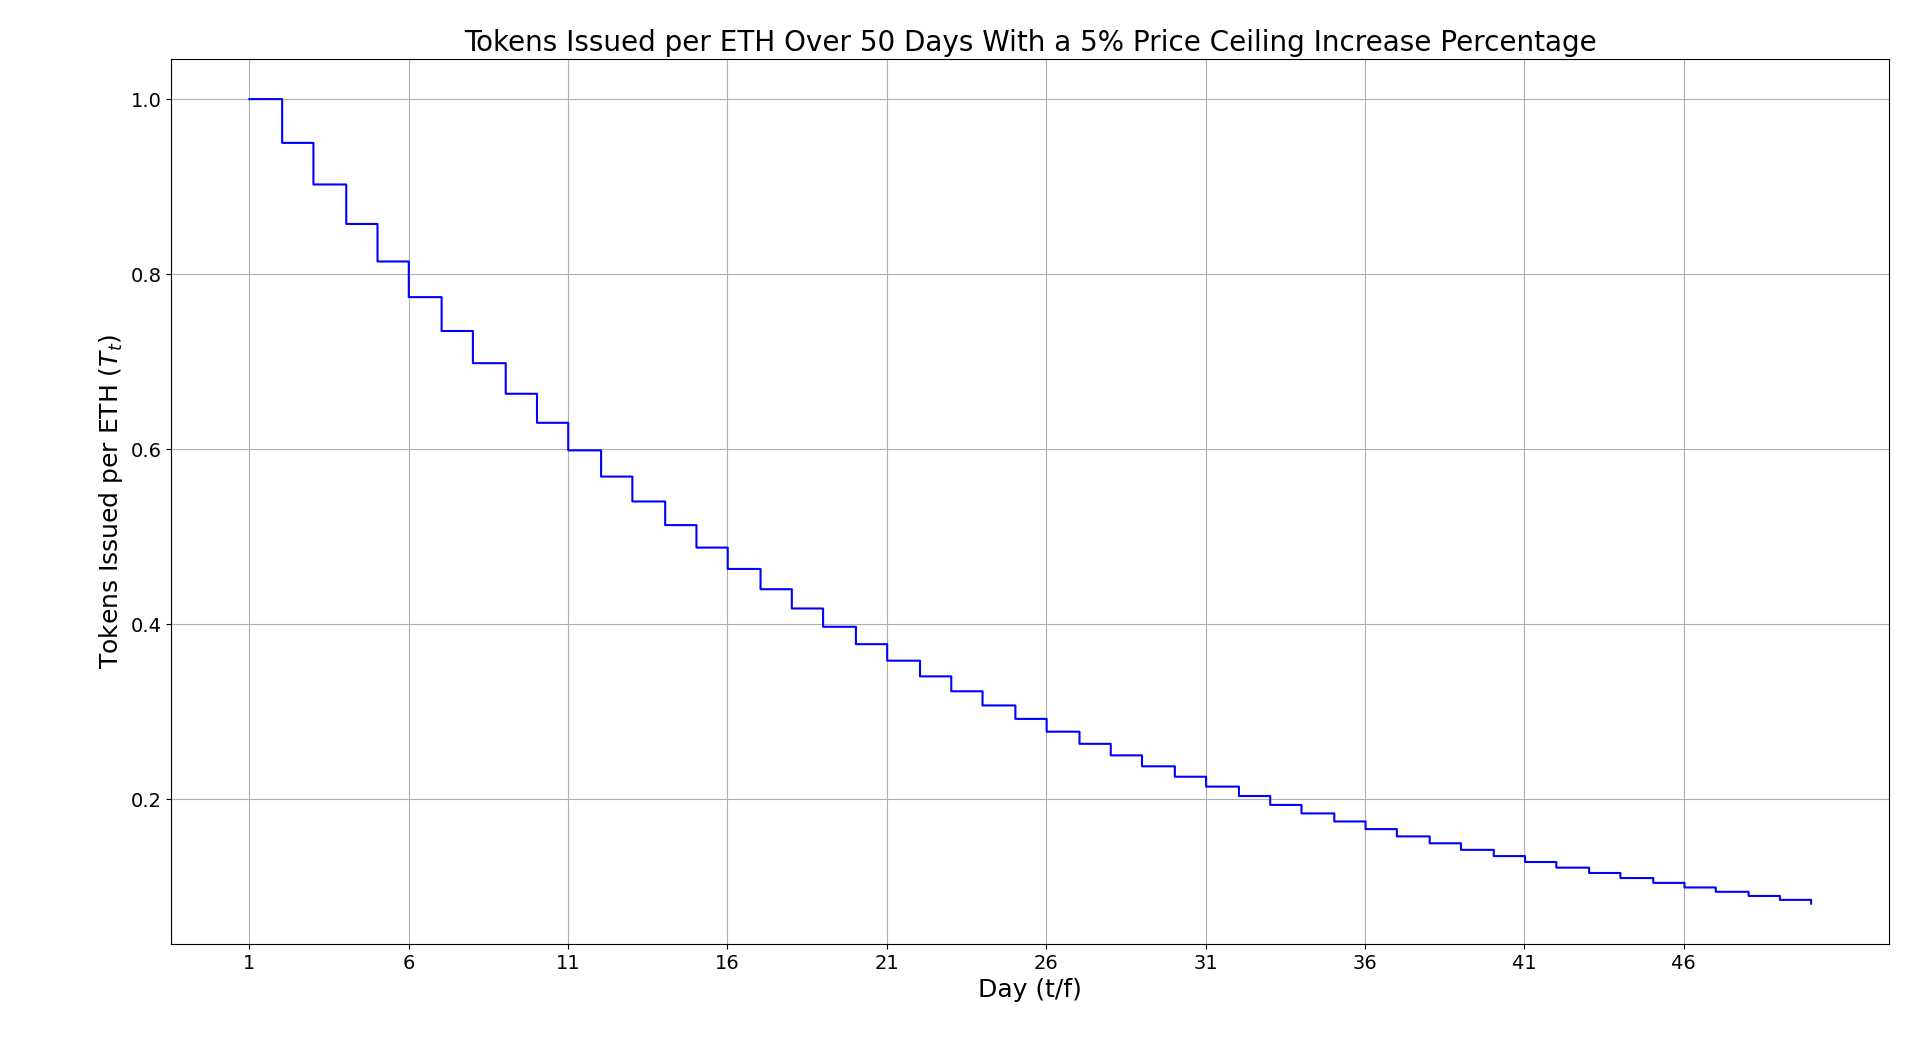
\includegraphics[width=\textwidth]{figures/single-ceiling-percentage.png}
   \caption{This figure shows how $T_t$ (the number of \$tokens issued per ETH at time $t$) varies over 50 days with a 5\% price ceiling increase percentage $(c = 0.05)$. Note that $T_t$ decreases rapidly at first, then more gradually as $T_n$ tends towards 0 over time. This figure assumes a price ceiling increase frequency of one day.}
\end{figure}


\begin{figure}[h]
  \centering
  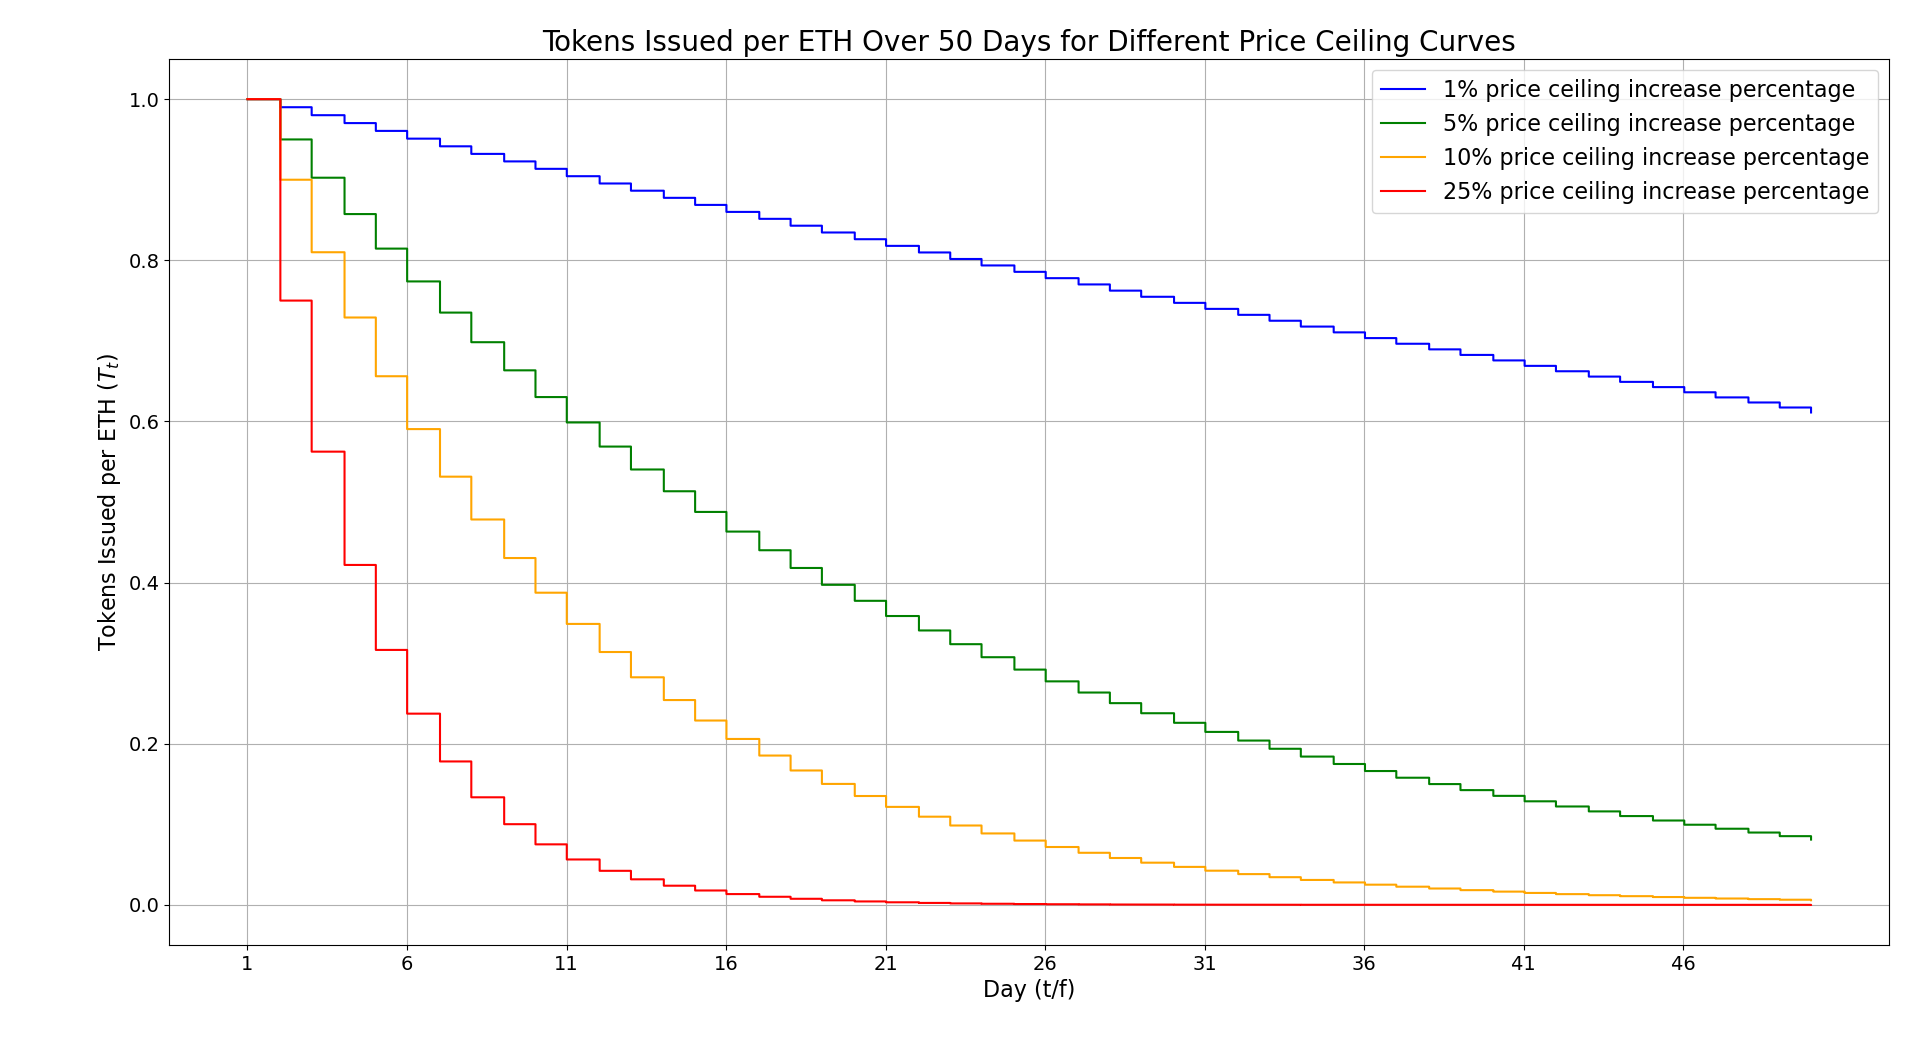
\includegraphics[width=\textwidth]{figures/multi-ceiling-percentages.png}
  \caption{This figure shows how $T_t$ varies over 50 days with 1\%, 5\%, 10\%, and 25\% price ceiling increase percentages $(c = 0.01, 0.05, 0.1, 0.25)$. Note that for greater price ceiling increase percenteages, $T_t$ tends towards 0 more quickly.}
\end{figure}

\subsection{Price Floor}

Anyone can destroy their \$tokens to reclaim ETH from the network. The amount of ETH they can reclaim is determined by the price floor, which is dynamically calculated based on the total \$token supply, the amount of ETH in the network, and a price floor tax intensity $i$ set by the network's creator. Unless the price floor tax intensity is 0 $(i = 0)$, destroying $n\%$ of tokens will reclaim less than $n\%$ of the network's ETH.\footnote{Unless $n = 100\%$} With a greater price floor tax intensity, more ETH stays in the network when tokens are destroyed, increasing the amount of ETH which can be reclaimed by other participants.

The price floor\footnote{Also see the interactive price floor on \href{https://www.desmos.com/calculator/9pewqesyj5}{Desmos}.} can be expressed as:

\begin{equation}
  V_r = \frac{V_t \cdot x}{s}\left(\left(1-i\right)+\frac{ix}{s}\right)
\end{equation}

where:
\begin{itemize}
  \item $V_r$ is the ETH value which gets reclaimed,
  \item $V_t$ is the total amount of ETH in the network,
  \item $s$ is the total \$token supply,
  \item $i$ is the price floor tax intensity (expressed as a decimal), and
  \item $x$ is the number of \$tokens being burned.
\end{itemize}

Unless $i$ is 0, as more \$tokens are destroyed (in other words, the larger $x$ is), more ETH is reclaimed per token.\footnote{If $i$ is 0, the price floor will be linear, and each \$token will yield the same amount of ETH when destroyed.} This means the first participants to destroy their \$tokens receive less ETH per \$token than participants who destroy their \$tokens later. This incentivizes participants to stay in the network longer in order to increase the amount of ETH they can reclaim.

\begin{figure}[ht]
  \centering
  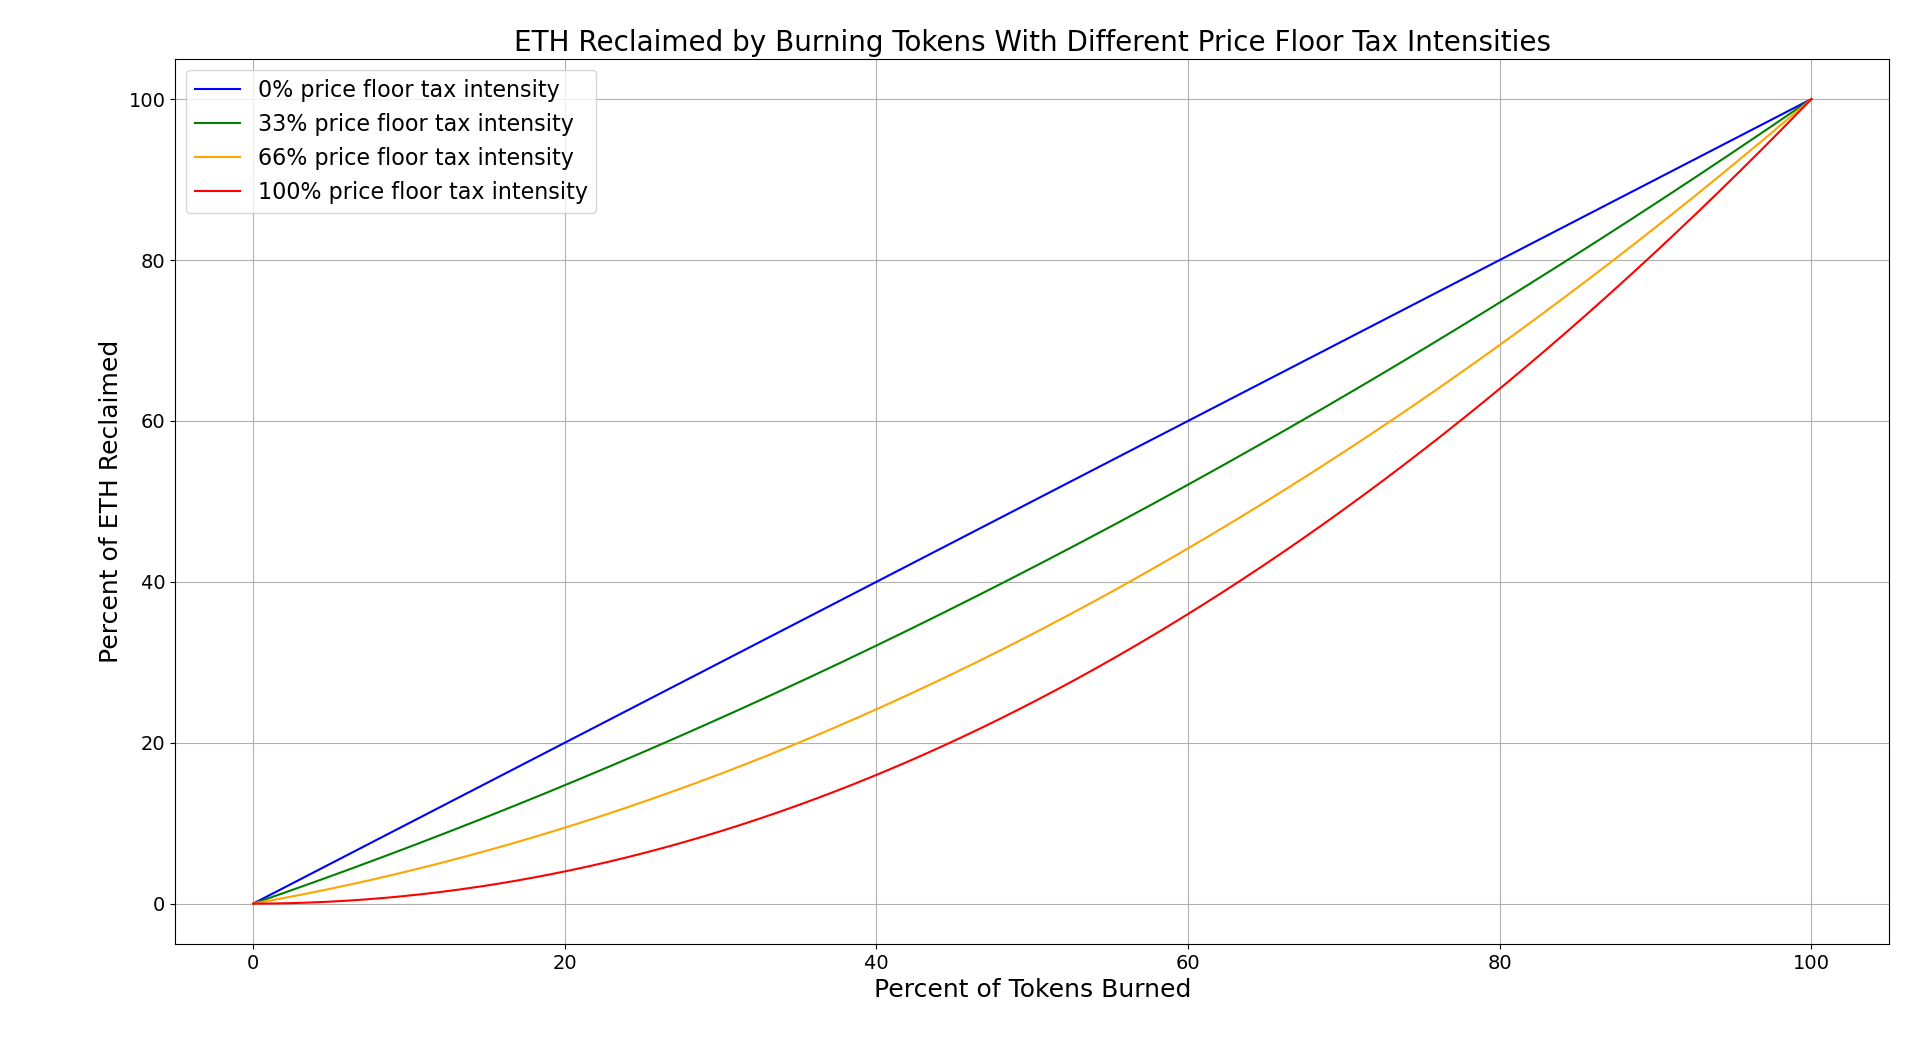
\includegraphics[width=\textwidth]{figures/multi-floor-intensities.png}
  \caption{This figure shows several price floors with price floor tax intensities of 0\%, 33\%, 66\%, and 100\% $(i = 0, 0.33, 0.66, 1)$. The $x$ axis represents the percentage of the total \$token supply being destroyed, and the $y$ axis represents the percentage of the network's ETH which is reclaimed. Note that with a 0\% price floor tax intensity $(i = 0)$, reclaim amounts scale linearly with respect to the number of tokens being destroyed---a network participant which destroys 1\% of the total token supply receives 1\% of the network's ETH. The larger the price floor tax intensity $i$, the less ETH earlier reclaimers receive.}
\end{figure}

For a participant to maximize their financial return under the shareholder value model, they must ``time the market'', selling their equity in a company at the time when the market considers it to be most valuable. This may not line up with the company's intrinsic value, as markets frequently overvalue or undervalue companies based on social trends, investor hype, and other extrinsic factors. In contrast, \textit{the greatest loss a participant can incur under a Revnet model is the difference between the price ceiling and price floor at the time they purchase \$tokens}. As \$tokens are created or destroyed, the price floor will continue to rise. Participants do not have to worry about the value of their tokens going to zero, and in most cases, to maximize their return, they only have to continue holding their tokens. Revnets make it easier for participants to be intelligent market actors.

\section{Applications}

Revnets can receive funds from token purchasers or from ongoing revenues. In practice, most Revnets will likely rely on token purchases to bootstrap early development, and transition to sustainable funding from revenues as the Revnet launches their product and achieves scale. Because of the bounds on the price window, Revnet token prices are generally stable and predictable, making them useful for projects with a long-term orientation. Revnets can leverage their boost to encourage early growth of the network and overcome the ``cold start'' effect new ventures often encounter. Revnets are particularly beneficial for applications that leverage network effects, where the service or product's value increases with greater participant involvement. Revnets are most capable of accomplishing complex coordinated tasks while the boost is active and can be strategically deployed by the boost operator.

Revnets excel in scenarios where individual contributors, even when isolated, can meaningfully contribute to the end product. An anonymous individual can write pages for an online encyclopedia or provide reviews for local businesses, making it feasible to coordinate hundreds or thousands of contributors to a project. Revnets are not as well-suited to endeavors which require ongoing support from a centralized, hierarchical structure. For instance, a Revnet would likely struggle to compete with a large-scale manufacturing company or to orchestrate the construction of complex infrastructure projects.

\subsection{Overcoming Existing Network Effects}

In spaces where products rely on user-driven network effects, newcomers often struggle to secure market share. Even when a newcomer has a technically better product, it is difficult to compete with established networks of users and content. This problem reinforces itself: a newcomer's lack of users makes their product or platform less useful, making it harder to attract users. This cold start problem can be overcome with a properly configured Revnet which incentivizes early users.

Google Maps is popular, but comes with several downsides: it is proprietary, its API is expensive, it has limited offline support, and it lacks data privacy. OpenStreetMap, an open-source alternative, addresses many of these concerns, but lacks in user-generated reviews and address labels, making it impractical for most. If OpenStreetMap or a project like it were to use a Revnet model, early participants would receive more of the Revnet's tokens, incentivizing them to leave more reviews and label more addresses. The boost could also be deployed to reward early contributors. If well-executed, this could generate enough content to make OpenStreetMap a viable option for users who care about data privacy or offline support---those users would continue to generate content, and eventually OpenStreetMap could gather enough data to be a viable option for all users.

Similarly, alternative social media platforms, such as Mastodon, and protocols like XMPP or Gemini could effectively generate early network momentum as Revnets. These Revnets wouldn't necessarily have to monetize the platform or protocol themselves---in line with existing corporate models, they could derive revenue from advertising or the sale of premium services and products, such as web hosting or educational resources. 

Currently, network effects are often overcome by using investor funding to subsidize a product, undercutting competition. Once these products secure a dominant market position, prices are increased, trapping users in a more expensive ecosystem. Revnets provide an alternative to this model, driving the cost per consumer down, or into profitability as the network achieves scale.

\subsection{Governance}

Revnet tokens adhere to the \texttt{ERC20Votes} standard, meaning they can be used in conjunction with governance tools like Snapshot and Governor Bravo for offchain or onchain token voting. Importantly, Revnet governance cannot control the allocation of the network's funds, as funds only leave the network according to the Revnet's pre-defined rules. This means Revnets are not subject to a wide range of governance attacks, hostile takeovers, and misaligned incentives which affect DAOs and other governance structures. Revnets can effectively govern DeFi protocols, software projects, and other efforts across distributed communities. Revnet mechanisms encourage long-term orientation and distribute tokens accordingly, encouraging favorable governance outcomes.

\subsection{Gated Networks}

Ethereum wallets offer straightforward sign-in support for web applications, making Revnets a strong fit for token-gated platforms. Since participants have access to the growth of a Revnet-driven platform, they're more likely to use the platform and recommend it to others. This is a major advantage for platforms which rely on user-generated content.

\begin{table}[h]
  \centering
  \begin{tabular}{|l|l|}
    \hline \textbf{Category} & \textbf{Examples} \\
    \hline Traditional social media. & Twitter, Instagram, and Facebook. \\
    \hline Forums and real-time chat services. & Reddit, Discord, and IRC. \\
    \hline Video and streaming services. & YouTube, Soundcloud, and Twitch. \\
    \hline Review and rating platforms. & Yelp, TripAdvisor, and Rotten Tomatoes. \\
    \hline News and Blogging platforms. & Medium, Mirror, and Tumblr. \\
    \hline Open or volunteer research and science. & Folding@home, BOINC, and LHC@home. \\
    \hline DeFi platforms which rely on user liquidity. & Uniswap, Compound, and Stargate. \\
    \hline
  \end{tabular}
  \caption{Types of platforms which rely on user-generated content and current examples.}
\end{table}

All else being equal, users are more likely to put value into a platform which allows them to receive a portion of future growth over one which doesn't. Community ownership also prevents the platform from switching to a more extractive business model once it achieves scale, a frequent misalignment between users and platforms. Individual content creator can also deploy Revnets, and allow token holders to access exclusive material. Content creators can also use token voting to guide the direction of future projects.

\section{Contract Implementation}

Revnets are implemented as Solidity smart contracts, and are intended for use on Ethereum and L2s. Revnets extend the Juicebox\footnote{See the \href{https://docs.juicebox.money}{Juicebox Docs}.} protocol, leveraging its discount rate logic for price ceiling calculations, its redemption logic for price floor calculations, and its reserved rate logic for boost calculations.

While a Revnet's token price is between its price ceiling and price floor, payments are routed to a Uniswap v3 liquidity pool by a Buyback Delegate\footnote{See the Buyback Delegate contracts on \href{https://github.com/jbx-protocol/juice-buyback}{GitHub}.} contract if possible. The Buyback Delegate contract routes incoming payments to the Uniswap pool if doing so would yield more tokens than a payment into the network would create.

Each Revnet is a Juicebox project, which is deployed, owned, and administered by a deployer contract. Our initial implementation includes a basic deployer, a deployer which includes pay delegates\footnote{See the \href{https://docs.juicebox.money/dev/learn/glossary/delegate/}{delegate documentation}.} to be called when the Revnet is paid, and a deployer which allows the Revnet to mint tiered ERC-721 NFTs when people pay it. These deployers are available on \href{https://github.com/rev-net/revnet-contracts}{GitHub}.

\subsection{Accounting Types}\label{sec:accounting_types}

Revnets have the option to use USD-based accounting based on a Chainlink ETH price oracle. With USD-based accounting, payers receive 1 network token per USD worth of ETH under the network's initial conditions. For instance, if the ETH price is 1,000 USD, paying 1 ETH into the network will create 1,000 tokens. Revnets can manage accounting with any price feed available on the \texttt{JBPrices} contract.\footnote{See the \href{https://docs.juicebox.money/dev/api/contracts/jbprices/}{\texttt{JBPrices} documentation}.}

\subsection{L2s}

Revnets communities will be able to utilize a collection of contracts to route funds between and coordinate across Ethereum mainnet and L2s. These contracts are currently under development and are available on \href{https://github.com/Bananapus}{GitHub}.

\section{Conclusion}

Revnets introduce a promising new growth model, with intrinsic incentives for early participation and enduring engagement. Utilizing unowned smart contracts, they avoid many of the trust and governance hurdles often faced by DAOs and other frameworks. By establishing a predictable token economy with a clear mechanism for value distribution and appreciation, Revnets enable sustainable user-centric networks. This model is particularly well-suited for ventures which thrive on network effects and community engagement, offering a solution to the cold start problem that many new ventures encounter.

With a predictable price ceiling, floor, and window, Revnets promote long-term participation and reduce, or often even benefit from the adversarial impact of market speculation which frequently impacts other token economies. Their utility extends beyond just being a medium of exchange or a store of value---they act as a catalyst for a wide range of community-driven platforms. In a digital age where user-generated value is essential to network growth, Revnets could play a pivotal role in redefining how value is created, distributed, and sustained. Through Revnets, we envision a future where the divide between users, builders, and investors is blurred, and where communities drive the value and direction of the networks they belong to.

\end{document}
